\documentclass[tikz]{standalone}
\usepackage{pgfplots}
\pgfplotsset{compat=1.17}
\usepgfplotslibrary{external}
\usepgfplotslibrary{groupplots}
\usepgfplotslibrary{fillbetween}
\usetikzlibrary{fadings}
\begin{document}
\tikzsetnextfilename{figures/tex/mab-samples.pdf}
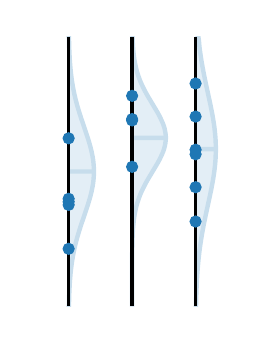
\begin{tikzpicture}
\begin{axis}[axis lines={none}, height={5cm}, width={4cm}, xmin={-1.5}, xmax={1.5}, ymin={-3}, ymax={3}, clip mode={individual}]
    \node at (-1.5,-3) {};
    \node at (1.5,-3) {};
    \node at (1.5,3) {};
    \node at (-1.5,3) {};
    \begin{scope}
    [transparency group, opacity={0.25}] \clip(-1.5,-3) rectangle (1.5,3);
    \draw
    [ultra thick, draw={rgb,1:red,0.1216;green,0.4667;blue,0.7059}] plot coordinates {
    (-1.0, 0.0)  (-0.6010577195985674, 0.0)
    };
    \draw
    [ultra thick, draw={rgb,1:red,0.1216;green,0.4667;blue,0.7059}] plot coordinates {
    (0.0, 0.75)  (0.5319230405352436, 0.75)
    };
    \draw
    [ultra thick, draw={rgb,1:red,0.1216;green,0.4667;blue,0.7059}] plot coordinates {
    (1.0, 0.5)  (1.319153824321146, 0.5)
    };
    \draw
    [ultra thick, draw={rgb,1:red,0.1216;green,0.4667;blue,0.7059}, fill={rgb,1:red,0.1216;green,0.4667;blue,0.7059}, fill opacity={0.5}] plot [smooth] coordinates {
    (-1.0, -3.0)  (-0.995568151588062, -3.0)  (-0.9909064374984089, -2.75)  (-0.9824716995064314, -2.5)  (-0.9682603481643326, -2.25)  (-0.946009033486812, -2.0)  (-0.9137226811734884, -1.75)  (-0.8704824043341083, -1.5)  (-0.8173509146109781, -1.25)  (-0.7580292754808566, -1.0)  (-0.6988625678451956, -0.75)  (-0.6479346732357005, -0.5)  (-0.6133318831971508, -0.25)  (-0.6010577195985674, 0.0)  (-0.6133318831971508, 0.25)  (-0.6479346732357005, 0.5)  (-0.6988625678451956, 0.75)  (-0.7580292754808566, 1.0)  (-0.8173509146109781, 1.25)  (-0.8704824043341083, 1.5)  (-0.9137226811734884, 1.75)  (-0.946009033486812, 2.0)  (-0.9682603481643326, 2.25)  (-0.9824716995064314, 2.5)  (-0.9909064374984089, 2.75)  (-0.995568151588062, 3.0)  (-1.0, 3.0)
    };
    \draw
    [ultra thick, draw={rgb,1:red,0.1216;green,0.4667;blue,0.7059}, fill={rgb,1:red,0.1216;green,0.4667;blue,0.7059}, fill opacity={0.5}] plot [smooth] coordinates {
    (0.0, -3.0)  (1.9822926863123968e-6, -3.0)  (9.928061160839987e-6, -2.75)  (4.4494483194184566e-5, -2.5)  (0.00017844030101984716, -2.25)  (0.0006403608688277609, -2.0)  (0.0020563719950548068, -1.75)  (0.005909131215917344, -1.5)  (0.015194648031729922, -1.25)  (0.03496251879161264, -1.0)  (0.07198795535091741, -0.75)  (0.13263618505699823, -0.5)  (0.2186800995679915, -0.25)  (0.32262763269219114, 0.0)  (0.425930674029803, 0.25)  (0.5031776369239909, 0.5)  (0.5319230405352436, 0.75)  (0.5031776369239909, 1.0)  (0.425930674029803, 1.25)  (0.32262763269219114, 1.5)  (0.2186800995679915, 1.75)  (0.13263618505699823, 2.0)  (0.07198795535091741, 2.25)  (0.03496251879161264, 2.5)  (0.015194648031729922, 2.75)  (0.005909131215917344, 3.0)  (0.0, 3.0)
    };
    \draw
    [ultra thick, draw={rgb,1:red,0.1216;green,0.4667;blue,0.7059}, fill={rgb,1:red,0.1216;green,0.4667;blue,0.7059}, fill opacity={0.5}] plot [smooth] coordinates {
    (1.0, -3.0)  (1.006332361266384, -3.0)  (1.0108663753869485, -2.75)  (1.0179156242358742, -2.5)  (1.028379674276985, -2.25)  (1.0431927732105504, -2.0)  (1.0631601266407154, -1.75)  (1.0887366677435644, -1.5)  (1.119781972508596, -1.25)  (1.1553488439865705, -1.0)  (1.1935765796153146, -0.75)  (1.2317532422091861, -0.5)  (1.2665796823134396, -0.25)  (1.2946161122426587, 0.0)  (1.3128341551803646, 0.25)  (1.319153824321146, 0.5)  (1.3128341551803646, 0.75)  (1.2946161122426587, 1.0)  (1.2665796823134396, 1.25)  (1.2317532422091861, 1.5)  (1.1935765796153146, 1.75)  (1.1553488439865705, 2.0)  (1.119781972508596, 2.25)  (1.0887366677435644, 2.5)  (1.0631601266407154, 2.75)  (1.0431927732105504, 3.0)  (1.0, 3.0)
    };
    \end{scope}
    \draw[black, very thick] ({axis cs:-1,0}|-{rel axis cs:0,1}) -- ({axis cs:-1,0}|-{rel axis cs:0,0});
    \draw[black, very thick] ({axis cs:0,0}|-{rel axis cs:0,1}) -- ({axis cs:0,0}|-{rel axis cs:0,0});
    \draw[black, very thick] ({axis cs:1,0}|-{rel axis cs:0,1}) -- ({axis cs:1,0}|-{rel axis cs:0,0});
    \addplot[only marks, color={rgb,1:red,0.1216;green,0.4667;blue,0.7059}]
        coordinates {
            (-1.0,0.7396206598864331)
            (-1.0,-0.7445071021408705)
            (-1.0,-0.6085075626113596)
            (-1.0,-1.7234565107957984)
            (-1.0,-0.6756156074023714)
        }
        ;
    \addplot[only marks, color={rgb,1:red,0.1216;green,0.4667;blue,0.7059}]
        coordinates {
            (0.0,1.167484750027598)
            (0.0,0.10381164512481122)
            (0.0,1.1385638307985484)
            (0.0,1.68617235607297)
        }
        ;
    \addplot[only marks, color={rgb,1:red,0.1216;green,0.4667;blue,0.7059}]
        coordinates {
            (1.0,1.9613911936905772)
            (1.0,0.38372765017046945)
            (1.0,-1.115504071589022)
            (1.0,0.4851584297344153)
            (1.0,1.223914307080334)
            (1.0,-0.3503890587311874)
        }
        ;
\end{axis}
\end{tikzpicture}
\end{document}
